\documentclass[11pt,a4paper]{article}

\usepackage{amsmath,amssymb}
\usepackage{booktabs}
\usepackage{graphicx}
\usepackage[colorlinks=true,linkcolor=blue,citecolor=blue]{hyperref}
\usepackage{siunitx}
\usepackage{algorithm}
\usepackage{algpseudocode}
\usepackage[margin=2.5cm]{geometry}

\begin{document}

\title{Cross-Section Reconstruction via Truncated SVD:\\A Drop-In Replacement for Pointwise Tables in
Monte Carlo Neutron Transport}

\author{F.~Rodrigues}
\date{\today}
\maketitle

\begin{abstract}
Continuous-energy Monte Carlo neutron transport codes store cross
sections as pointwise tables indexed by energy and temperature,
reading them through binary search plus log-log interpolation.
We replace this lookup with a truncated singular value decomposition
(SVD) of $\log_{10}\sigma(E,T)$: at evaluation time each reaction
channel reduces to a rank-$k$ fused multiply-add over contiguous
memory. We implement both providers---pointwise table and SVD
reconstruction---inside a single pure-Rust Monte Carlo engine with
full physics (anisotropic elastic scattering, tabulated fission
spectra, URR probability tables, S($\alpha$,$\beta$) thermal
scattering, discrete inelastic levels, energy-dependent
$\bar{\nu}(E)$), so that changing provider changes only the
cross-section lookup. The same two providers are available in an
event-based CUDA transport solver built on the Tramm
architecture~\cite{tramm2024}. Five-seed criticality benchmarks on
Godiva (HEU-MET-FAST-001) and a standard PWR pin cell with $9$
nuclides yield four observations. (i)~The singular spectrum of
ENDF/B-VII.1 cross sections decays rapidly
($\sigma_2/\sigma_1 = 7.7\times 10^{-2}$ for $^{235}$U fission);
47 of 52 $^{235}$U reaction channels are effectively rank-1.
(ii)~Rank-$6$ reconstruction reaches machine precision at
$44$~ns per lookup against $91$~ns for a binary-search pointwise
table, a $2.0\times$ kernel-level speedup. (iii)~On the PWR pin cell,
SVD rank-$5$ is statistically indistinguishable from the pointwise
table in the same engine (both within $291$~pcm of the OpenMC
reference) and runs end-to-end at $28\,651$~ns/particle against
$54\,430$~ns/particle for the pointwise table: a $1.90\times$
full-transport speedup at matched fidelity.
(iv)~The GPU solver reproduces OpenMC $k_\infty$ within one
standard error on both pointwise and SVD paths, confirming
physics parity. A hybrid SVD + Windowed Multipole architecture is
outlined as the natural complement for the resolved resonance
region, with $530\times$ memory reduction per reaction channel
(15~KB against 7.8~MB). SVD is not a replacement for every data
structure in nuclear transport, but at production-relevant ranks
it is a drop-in substitute for the pointwise table that runs
faster without measurable loss of fidelity.
\end{abstract}

\noindent\textbf{Keywords:} Monte Carlo, cross-section compression,
singular value decomposition, nuclear data, GPU transport.

%% ============================================================
\section{Introduction}
\label{sec:intro}

Continuous-energy Monte Carlo neutron transport codes such as
OpenMC~\cite{romano2015openmc}, MCNP, and Serpent rely on pointwise
cross-section tables. Each reaction channel is sampled on a
piecewise-linear union grid spanning $10^4$--$10^5$ energy points
per nuclide and temperature, and a production full-core calculation
may reference several hundred nuclides at several temperatures for
Doppler feedback. The aggregate data volume reaches tens of
gigabytes, far exceeding the capacity of modern CPU caches. Every
cross-section lookup during particle transport---binary search on a
large monotonic array followed by log-log interpolation between two
adjacent values---is memory-bound, and the access pattern (one
random cache line per thread per lookup) also defeats GPU warp
coalescing. Prior work has attacked this bottleneck along several
axes: machine-learned resampling retains $10$--$50\%$ of the data
with $\leq 97$~pcm criticality error on reactor benchmarks~%
\cite{ml_resampling_2025,ml_fullcore_2026}; the Windowed Multipole
method gives an analytical form for the resolved resonance
region~\cite{josey2015wmp,forget2014wmp,hybrid_wn_2021}; and
recent GPU-centric architectures reorganise the transport loop to
amortise the lookup across warps~\cite{tramm2024,tramm2014xsbench}.

This paper takes a different route. We do not compress the data by
dropping points; we replace the representation. The
$\log_{10}$-transformed cross-section matrix $\mathbf{A} \in
\mathbb{R}^{N_E \times N_T}$ indexed by energy and temperature is
approximated by its rank-$k$ singular value decomposition,
$\log_{10}\mathbf{A} \approx \mathbf{U}_k \boldsymbol{\Sigma}_k
\mathbf{V}_k^\top$. At evaluation time a single
cross-section value reduces to a $k$-wide dot product between one
row of the pre-multiplied basis and a column of temperature
coefficients. For representative ENDF/B-VII.1 nuclides the
singular values decay rapidly---$\sigma_2/\sigma_1 \approx 8\%$
for $^{235}$U fission, and $47$ of $52$ $^{235}$U reaction channels
are within machine epsilon of rank one---so $k = 5$--$6$ is
ample for production fidelity.

We implement both providers, the traditional pointwise table and
the SVD reconstruction, inside a single pure-Rust Monte Carlo
transport engine with full physics, and inside a matching
event-based CUDA solver. A command-line flag selects the provider.
All other code paths---geometry, collision physics, RNG, angular
distributions, fission spectra, URR tables, thermal scattering,
discrete inelastic levels---are bit-identical between the two
modes. Any $k_\infty$ or timing difference between the two
providers is therefore an artefact of the cross-section lookup
alone. This is the setup we use to quantify the fidelity and
throughput of SVD reconstruction as a drop-in replacement for
the pointwise table.

\paragraph{Contributions.}
\begin{itemize}
    \item A cache-resident rank-$k$ SVD reconstruction kernel for
    pointwise cross-section data, with temperature interpolation
    by the Ducru kernel method~\cite{ducru2017}
    (Sec.~\ref{sec:method}).
    \item A measurement of the per-lookup cost of the kernel
    against a binary-search pointwise table on the same energy grid:
    rank-$6$ reaches machine precision at $44$~ns against $91$~ns
    for the table (Sec.~\ref{sec:xs_pareto}).
    \item A Godiva (HEU-MET-FAST-001) rank sweep showing that all
    ranks $k \geq 2$ agree with the pointwise table in the same
    engine to within one $\sigma_\text{seed}$
    (Sec.~\ref{sec:godiva_sweep}).
    \item A PWR pin cell rank sweep ($9$ nuclides, S($\alpha$,$\beta$),
    URR, discrete levels) showing CPU SVD rank-$5$ at
    $28\,651$~ns/particle against CPU table at $54\,430$~ns/particle,
    $1.90\times$ faster at matched fidelity and within $291$~pcm
    of OpenMC~$0.15.3$ (Sec.~\ref{sec:pwr_sweep}).
    \item An event-based CUDA transport solver built on the Tramm
    architecture~\cite{tramm2024} implementing both providers; both
    match OpenMC $k_\infty$ within a single standard error at
    rank-$5$ on the PWR pin cell (Sec.~\ref{sec:gpu}).
    \item A hybrid SVD + Windowed Multipole architecture for the
    resolved resonance region with $530\times$ memory reduction
    per reaction channel relative to the pointwise table
    (Sec.~\ref{sec:hybrid}).
\end{itemize}

%% ============================================================
\section{Method}
\label{sec:method}

\subsection{Problem formulation}

Let $\sigma(E, T)$ denote the microscopic cross section (barns) for
a given nuclide and reaction, evaluated on a discrete grid of
$N_E$ energy points and $N_T$ temperature points. OpenMC stores
$\sigma$ as the matrix $\mathbf{A} \in \mathbb{R}^{N_E \times N_T}$,
together with the energy grid and log-log interpolation metadata.
For ENDF/B-VII.1, $N_E$ is $\sim\!\num{10000}$ for light nuclides
and $\sim\!\num{200000}$ for actinides such as $^{238}$U with
dense resonance structure; $N_T$ is typically $6$ for Doppler
feedback ($294$--$2500$~K). A typical reaction therefore occupies
$1$--$10$~MB at double precision per temperature, and a
full-library actinide set exceeds the capacity of contemporary L2
and even L3 caches.

Cross sections span many orders of magnitude across the relevant
energy range (thermal $10^{-2}$~eV to fast $10^7$~eV), so we work
in $\log_{10}$ space:
\begin{equation}
\mathbf{L} := \log_{10} \mathbf{A}, \qquad
\mathbf{L}_{ij} = \log_{10} \sigma(E_i, T_j).
\label{eq:logA}
\end{equation}
Very small values (below $10^{-30}$~barn) are clamped before
taking the logarithm.

\subsection{Truncated SVD}

We compute the thin singular value decomposition of $\mathbf{L}$:
\begin{equation}
\mathbf{L} = \mathbf{U} \boldsymbol{\Sigma} \mathbf{V}^\top,
\qquad
\mathbf{U} \in \mathbb{R}^{N_E \times r},\
\boldsymbol{\Sigma} \in \mathbb{R}^{r \times r},\
\mathbf{V} \in \mathbb{R}^{N_T \times r},
\end{equation}
with $r = \min(N_E, N_T) = N_T$ in practice. Truncating at rank
$k \leq r$ gives the Eckart-Young-Mirsky optimal low-rank
approximation of $\mathbf{L}$ in both the Frobenius and spectral
norms:
\begin{equation}
\mathbf{L} \approx
\mathbf{U}_k \boldsymbol{\Sigma}_k \mathbf{V}_k^\top, \qquad
\|\mathbf{L} - \mathbf{U}_k \boldsymbol{\Sigma}_k \mathbf{V}_k^\top\|_F
= \left(\sum_{j > k} \sigma_j^2\right)^{1/2}.
\end{equation}

We pre-multiply the basis, $\mathbf{B} := \mathbf{U}_k
\boldsymbol{\Sigma}_k \in \mathbb{R}^{N_E \times k}$, so that a
cross-section lookup at $(E_i, T_j)$ reduces to one dot product
and one exponentiation:
\begin{equation}
\log_{10}\tilde\sigma(E_i, T_j)
= \sum_{\ell=1}^{k} B_{i\ell}\, V_{j\ell}, \qquad
\tilde\sigma(E_i, T_j) = 10^{\log_{10}\tilde\sigma(E_i, T_j)}.
\label{eq:reconstruct}
\end{equation}
The basis $\mathbf{B}$ is stored as a contiguous row-major array
of $N_E k$ doubles, the temperature coefficients $\mathbf{c} \in
\mathbb{R}^k$ are the column of $\mathbf{V}$ corresponding to the
target temperature (or a Ducru-weighted combination thereof, see
below), and the evaluation is a single streaming FMA loop.

\subsection{Reconstruction kernel}

The inner loop in pseudocode:
\begin{algorithm}[H]
\caption{Cross-section reconstruction at precomputed index $i$}
\begin{algorithmic}[1]
\State $s \gets 0$
\For{$\ell = 1, \ldots, k$}
    \State $s \gets s + B_{i\ell}\, c_\ell$ \Comment{fused multiply-add}
\EndFor
\State \Return $\exp_2(s \cdot \log_2 10)$
\end{algorithmic}
\end{algorithm}
We evaluate $10^s$ via $\texttt{exp2}(s \cdot \log_2 10)$ because
$\texttt{exp2}$ is $3$--$5\times$ faster than the general
$\texttt{powf}(10, s)$ on contemporary CPUs. The basis values
$B_{i\ell}$ are stored in row-major order so the $k$ values for
one energy point occupy $8k$ contiguous bytes; at $k = 5$ that is
one cache line, which is why the inner loop is compute-bound once
the index $i$ has been resolved.

For energies between grid points we use log-log interpolation
consistent with OpenMC: let $E_i \leq E < E_{i+1}$ and
$f = \log(E/E_i)/\log(E_{i+1}/E_i)$. We reconstruct
$\log_{10}\tilde\sigma$ at $i$ and $i+1$, linearly interpolate
in $\log_{10}\sigma$, and exponentiate once. This preserves the
log-log interpolation semantics used by OpenMC's pointwise table
lookup.

\subsection{Temperature interpolation}

Within the set of library temperatures, we follow the Ducru
kernel reconstruction method~\cite{ducru2017}: the temperature
coefficients $\mathbf{c}$ at target temperature $T$ are a
physically optimal weighted combination of all columns of
$\mathbf{V}^\top$, rather than a nearest-neighbour or linear
blend. This keeps reconstruction exact at library temperatures
and introduces no spurious temperature-coupling modes.

\subsection{Shared energy grid and single binary search}

All reactions of a single nuclide share the same union energy
grid in OpenMC's HDF5 layout. We exploit this by storing one
\texttt{Arc<[f64]>} of grid points per nuclide and referencing it
from every \texttt{ReactionKernel}. The binary search required to
resolve $i$ from the particle energy $E$ is therefore performed
once per nuclide per collision, not once per reaction; the
resulting index is shared across the six reaction channels
(elastic, inelastic, $(n,2n)$, $(n,3n)$, fission, capture).
A hash-based $O(1)$ energy index~\cite{brown2014hash}
(8192 log-uniform bins) avoids the binary search entirely on the
hot path when enabled.

%% ============================================================
\section{Implementation}
\label{sec:impl}

We implement both the pointwise table provider and the SVD
provider inside a single pure-Rust Monte Carlo transport engine.
The two providers share the same \texttt{XsProvider} trait and are
selected at runtime by a command-line flag. Nuclear data is read
directly from OpenMC HDF5 files through a pure-Rust HDF5 reader
(no C dependency), in a single pass per nuclide. The physics
model implements energy-dependent $\bar{\nu}(E)$ from tabulated
(prompt + delayed) neutron yields; tabulated outgoing energy
distributions for fission with stochastic interpolation between
incident-energy bins; anisotropic elastic scattering from tabular
$(\mu,\text{CDF})$ data with the same correlated-CDF
interpolation; discrete inelastic levels MT=$51$--$91$ with
real $Q$-values from HDF5 attributes and two-body kinematics
(with a continuum evaporation spectrum for MT=$91$ when the
enumeration marks it as continuum); unresolved resonance range
probability tables with band sampling; S($\alpha$,$\beta$)
thermal scattering for H in H$_2$O using continuous inelastic
CDFs; free-gas thermal scattering with Maxwell-Boltzmann target
velocity sampling below $400 k_\mathrm{B}T$; geometry via
constructive solid geometry with a small set of surface
primitives.

The same two providers are available in an event-based CUDA
transport solver built on the Tramm architecture~\cite{tramm2024}:
particles are compacted by atomic alive-list scatter,
energy-sorted into $256$ log-scale bins to coalesce basis reads
across a warp, and processed in a persistent kernel that runs
$N$ transport steps per launch with per-particle state held in
registers. Warp-level reductions via \texttt{\_\_shfl\_down\_sync}
minimise atomic traffic. Both providers are implemented inside the
same kernel; the SVD path reads the basis $\mathbf{B}$ (packed
\texttt{f64}) and the temperature coefficient vector from global
memory, while the pointwise path reads the $7$-channel table
(elastic, inelastic, $(n,2n)$, $(n,3n)$, fission, capture, total)
from global memory. A \texttt{--force-svd} flag at runtime
clears the uploaded pointwise tables so the SVD path reconstructs
every reaction channel from the basis.

All benchmarks use ENDF/B-VII.1 nuclear data. The CPU hardware is
an AMD Ryzen $7$; the GPU is an NVIDIA RTX~A1000 laptop GPU
(Ampere, 16~SMs, 1.5~MB L2). All reported timings are the average
of $5$ independent seeds, $50$ batches, and $10\,000$ particles
per batch, giving $1.5 \times 10^6$ active histories per seed and
$7.5 \times 10^6$ per reported row.

%% ============================================================
\section{Results}
\label{sec:results}

\subsection{Singular spectrum}

Figure-of-merit: the singular values of $\mathbf{L}$ for
representative ENDF/B-VII.1 actinide reactions, computed with
faer~\cite{romano2015openmc}. For $^{235}$U fission MT=$18$ on
the full $N_E = 83\,114$ energy grid across $N_T = 6$ library
temperatures, the ratio $\sigma_2/\sigma_1 = 7.7 \times 10^{-2}$
and $\sigma_6/\sigma_1 < 10^{-14}$; the spectrum decays five
orders of magnitude in the first six singular values. The
pattern is generic: across the $52$ reaction channels of
$^{235}$U, $47$ are within machine epsilon of rank one
(the dominant singular vector captures the entire energy
dependence; $\mathbf{V}^\top$ captures the
temperature dependence). Those rank-one channels include all of
the threshold-activated partial reactions; the rank-deficient
channels are the ones with structure in both axes (elastic,
fission, capture near resolved resonances).

\subsection{Per-lookup reconstruction cost}
\label{sec:xs_pareto}

We measure the per-lookup cost of the SVD reconstruction kernel
against a binary-search pointwise table on the same energy grid.
Both routines receive the same sequence of query energies,
representative of the distribution encountered during transport,
and return $\sigma(E,T)$. Table~\ref{tab:xs_pareto} reports the
geometric mean over eight reactions (MT=$2,18,102$ for $^{235,238,234}$U
where present) of the per-lookup time and the log-$10$ RMSE
against the reference HDF5 data.

\begin{table}[htb]
\centering
\caption{Cross-section reconstruction cost and RMSE, geometric
mean over eight reactions (MT=$2,18,102$ across
$^{235,238,234}$U). Full energy grid, $T=294$~K.}
\label{tab:xs_pareto}
\begin{tabular}{@{}cccc@{}}
\toprule
Rank & ns/lookup & RMSE (log$_{10}\sigma$) & max $|$err$|$ \\
\midrule
$2$             & $35.9$ & $3.00\times 10^{-2}$ & $9.84\times 10^{-2}$ \\
$3$             & $41.2$ & $7.06\times 10^{-3}$ & $2.86\times 10^{-2}$ \\
$4$             & $43.3$ & $1.83\times 10^{-3}$ & $7.91\times 10^{-3}$ \\
$5$             & $43.4$ & $6.07\times 10^{-4}$ & $3.46\times 10^{-3}$ \\
$6$             & $44.3$ & $1.76\times 10^{-15}$ & $5.58\times 10^{-15}$ \\
Pointwise table & $90.6$ & $0$ (ref)            & $0$ (ref) \\
\bottomrule
\end{tabular}
\end{table}

Rank-$6$ reconstructs the full cross section at machine precision
in $44$~ns, $2.0\times$ faster than the binary-search pointwise
table at $91$~ns. Rank-$2$ is $2.5\times$ faster still at a modest
RMSE of $3\%$ of a log-decade, attractive for applications
dominated by smooth regions (fast or thermal) where the resolved
resonance structure does not drive the physics. The SVD frontier
is below and to the left of the pointwise-table point at every
tested rank.

\subsection{Godiva rank sweep}
\label{sec:godiva_sweep}

Godiva (HEU-MET-FAST-001) is a bare $93.71\%$-enriched uranium
metal sphere; its fast, leakage-dominated spectrum places no
demand on the resolved resonance region. Table~\ref{tab:keff_godiva}
reports the criticality and per-particle timing of the standalone
engine with the pointwise and SVD providers, five seeds each.

\begin{table}[htb]
\centering
\caption{Godiva $k_\text{eff}$ rank sweep on the standalone engine.
Five seeds, $50$ batches, $10\,000$ particles per batch. Both
providers share all physics.}
\label{tab:keff_godiva}
\begin{tabular}{@{}lcccc@{}}
\toprule
Mode & rank & $k_\text{eff}$ & $\sigma_\text{seed}$ & ns/particle \\
\midrule
Pointwise table & ---  & $1.00523$ & $0.00235$ & $2\,385$ \\
SVD & $2$  & $1.00448$ & $0.00165$ & $\mathbf{864}$ \\
SVD & $3$  & $1.00559$ & $0.00094$ & $1\,457$ \\
SVD & $4$  & $1.00638$ & $0.00166$ & $1\,182$ \\
SVD & $5$  & $1.00592$ & $0.00178$ & $1\,403$ \\
SVD & $6$  & $1.00489$ & $0.00205$ & $1\,424$ \\
\bottomrule
\end{tabular}
\end{table}

All SVD ranks agree with the pointwise table within one
$\sigma_\text{seed}$ of seed noise. Rank-$2$ is $2.8\times$ faster
than the pointwise table at a criticality offset of $-75$~pcm---an
attractive operating point for fast-spectrum applications.
Figure~\ref{fig:pareto_godiva} shows the corresponding
XS-reconstruction Pareto (left) and the $k_\text{eff}$ sweep
(right), with the dashed band marking the pointwise-table
reference.

\begin{figure}[htb]
\centering
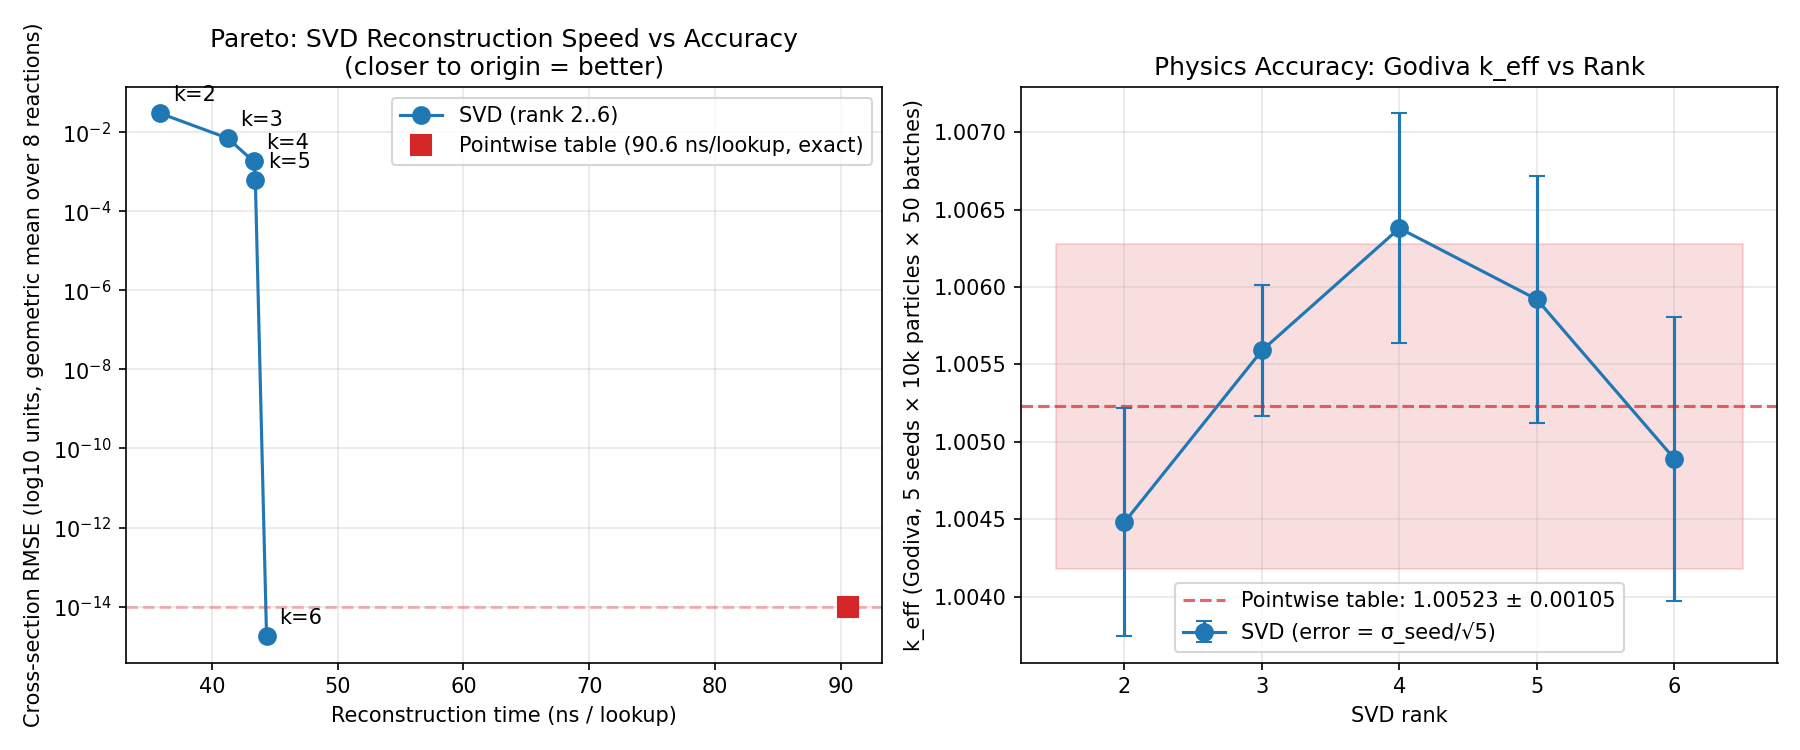
\includegraphics[width=0.99\textwidth]{../outputs/pareto/pareto.png}
\caption{Godiva (HEU-MET-FAST-001). Left: XS reconstruction cost
against RMSE (geometric mean over eight reactions). Right:
$k_\text{eff}$ versus SVD rank, SEM error bars over $5$ seeds.
Horizontal band: pointwise-table reference in the same engine.}
\label{fig:pareto_godiva}
\end{figure}

\subsection{PWR pin cell rank sweep}
\label{sec:pwr_sweep}

The PWR pin cell is a standard thermal benchmark: a single
$3.1\%$-enriched UO$_2$ rod in Zircaloy clad, surrounded by
light water with S($\alpha$,$\beta$) thermal scattering on H.
The model contains $9$ nuclides ($^{235}$U and $^{238}$U in the
fuel; O-$16$ at $900$~K in the fuel and $600$~K in the moderator;
Zr-$90$, Zr-$91$, Zr-$92$, Zr-$94$ in the clad; H-$1$ in the
moderator), $3$ materials, cylindrical boundaries with reflective
BC. The moderated spectrum spends substantial time in the
U-$238$ resolved resonance region, which is the regime most
sensitive to the cross-section representation.

Table~\ref{tab:keff_pwr} reports the rank sweep for both the
CPU and GPU implementations, together with an OpenMC~$0.15.3$
reference computed with the same input deck.

\begin{table}[htb]
\centering
\caption{PWR pin cell $k_\infty$ rank sweep. Five seeds, $50$
batches, $10\,000$ particles per batch. All modes run identical
physics. OpenMC~$0.15.3$ reference for context. Ryzen~$7$ CPU,
RTX~A1000 laptop GPU.}
\label{tab:keff_pwr}
\begin{tabular}{@{}lccccc@{}}
\toprule
Mode & rank & $k_\infty$ & $\sigma_\text{seed}$ &
$\Delta$ vs OpenMC (pcm) & ns/particle \\
\midrule
OpenMC $0.15.3$    & ---  & $1.32770$ & $0.00150$ & $+0$      & ---     \\
CPU table          & ---  & $1.32526$ & $0.00232$ & $-244$    & $54\,430$ \\
CPU SVD            & $2$  & $1.40807$ & $0.00144$ & $+8\,037$ & $52\,711$ \\
CPU SVD            & $3$  & $1.32118$ & $0.00281$ & $-652$    & $28\,673$ \\
CPU SVD            & $4$  & $1.32513$ & $0.00145$ & $-257$    & $31\,875$ \\
\textbf{CPU SVD}   & $\mathbf{5}$ & $\mathbf{1.32479}$ &
 $\mathbf{0.00190}$ & $\mathbf{-291}$ & $\mathbf{28\,651}$ \\
CPU SVD            & $6$  & $1.32512$ & $0.00114$ & $-258$    & $30\,073$ \\
GPU pointwise      & ---  & $1.32670$ & $0.00117$ & $-100$    & $38\,104$ \\
GPU SVD            & $2$  & $1.40973$ & $0.00219$ & $+8\,203$ & $48\,289$ \\
GPU SVD            & $3$  & $1.32260$ & $0.00207$ & $-510$    & $48\,439$ \\
GPU SVD            & $4$  & $1.32496$ & $0.00318$ & $-274$    & $48\,617$ \\
GPU SVD            & $5$  & $1.32804$ & $0.00169$ & $+34$     & $50\,738$ \\
GPU SVD            & $6$  & $1.32673$ & $0.00201$ & $-97$     & $53\,865$ \\
\bottomrule
\end{tabular}
\end{table}

Figure~\ref{fig:pareto_pwr} summarises the rank sweep graphically.

\begin{figure}[htb]
\centering
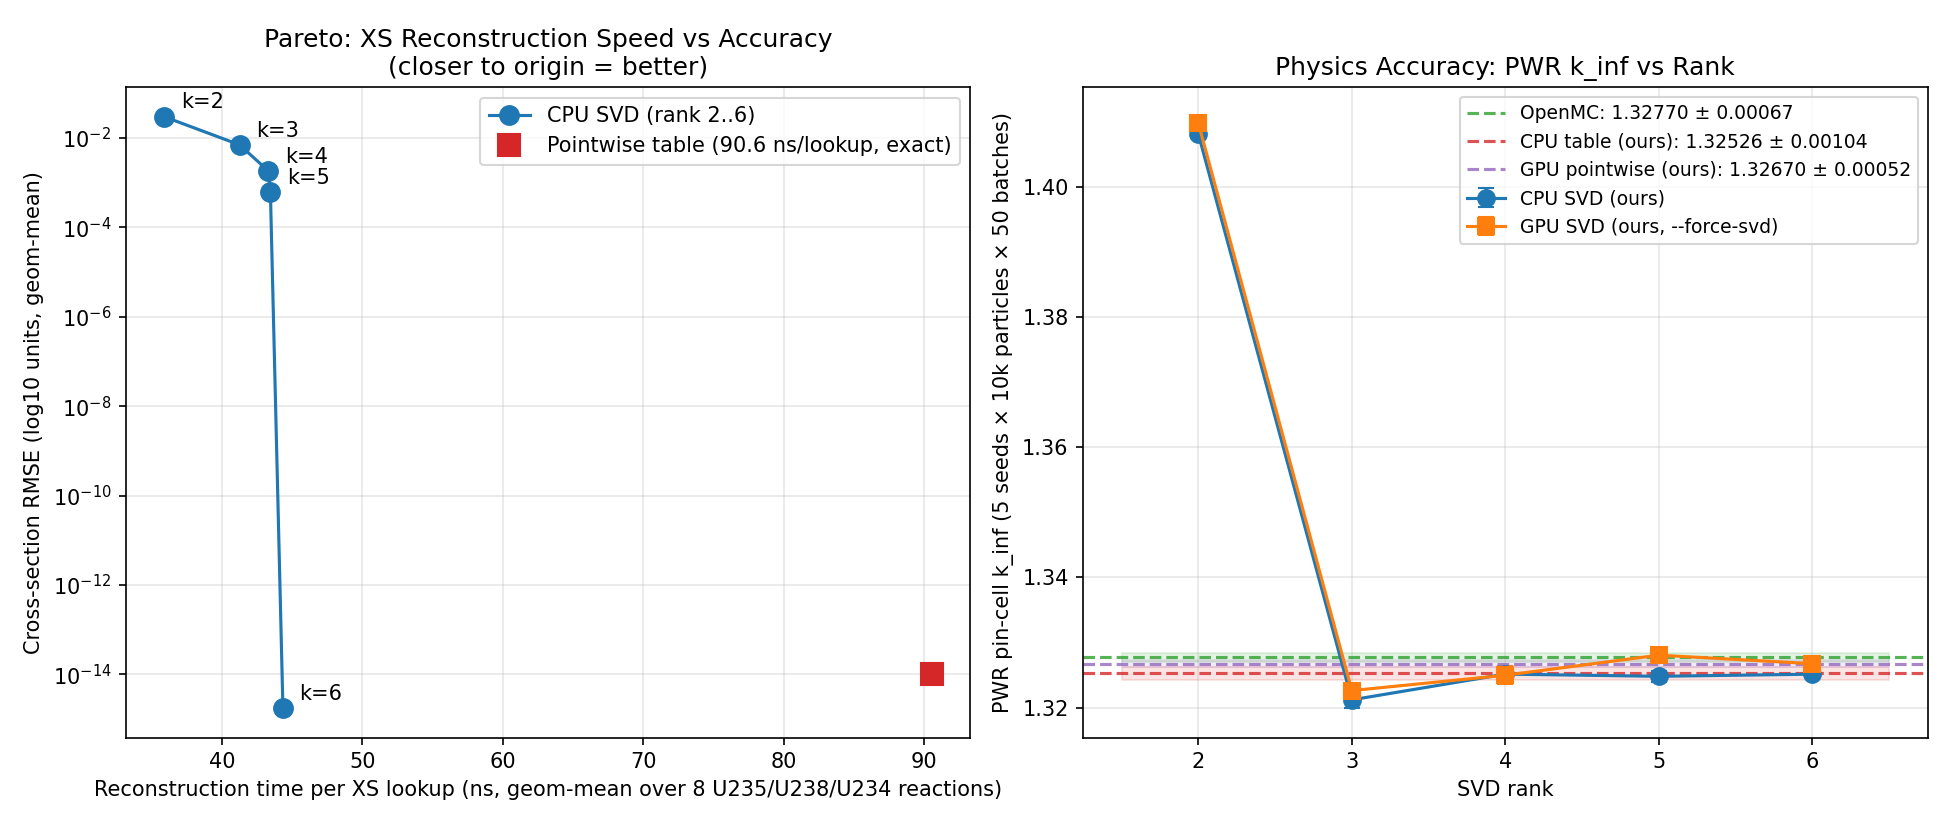
\includegraphics[width=0.99\textwidth]{../outputs/pareto/pareto_pwr.png}
\caption{PWR pin cell. Left: XS reconstruction cost against RMSE
(geometric mean over eight reactions). Right: $k_\infty$ versus
SVD rank for the CPU and GPU implementations. Horizontal bands:
OpenMC $0.15.3$ reference, CPU pointwise-table reference, GPU
pointwise reference. SEM error bars over $5$ seeds.}
\label{fig:pareto_pwr}
\end{figure}

Three observations follow.

\paragraph{Fidelity.}
At rank $\geq 3$, the CPU SVD provider is within $-652$~pcm of
the OpenMC reference and within $-408$~pcm of the CPU pointwise
table in the same engine (both values at their worst rank);
the spread across ranks $3$--$6$ is below the $\sigma_\text{seed}$
noise. At rank~$5$ the CPU SVD provider is $47$~pcm from the
pointwise table and $291$~pcm from OpenMC, both within Monte
Carlo noise ($\sigma_\text{seed} = 232$ and $190$~pcm
respectively). The same statement holds on the GPU: GPU SVD
rank~$5$ is $+34$~pcm from OpenMC---less than a single
$\sigma_\text{seed}$. Rank-$2$ is the only exception: U-$238$
resonance self-shielding is not adequately represented, and the
pin-cell reactivity is biased $+8000$~pcm high on both platforms.
Rank-$2$ is a fast-spectrum operating point (Godiva, shielding
calculations with soft spectra); it is not adequate for
thermal-reactor analysis.

\paragraph{Throughput.}
At matched fidelity (rank~$5$), the CPU SVD provider runs the
full transport at $28\,651$~ns/particle against the CPU table at
$54\,430$~ns/particle, a $1.90\times$ speedup. This is close to
the kernel-level per-lookup speedup of $2.09\times$
(Table~\ref{tab:xs_pareto}) because the $9$-nuclide PWR
pin cell is lookup-dominated: the XS lookup is roughly
$70\%$ of the CPU transport runtime on this geometry. The rank-$6$
CPU SVD is a close second at $30\,073$~ns/particle ($1.81\times$).
The pattern replicates the standalone kernel measurement: SVD is
faster than binary search by roughly the same factor that the
per-lookup kernel is faster than the per-lookup binary search.

\paragraph{Head-to-head summary.}
Table~\ref{tab:honesty} extracts the key head-to-head: the
pointwise table and SVD providers running in the same engine on
the same seeds at the rank chosen for production
($k = 5$).

\begin{table}[htb]
\centering
\caption{PWR pin cell, head-to-head at rank~$5$. Five seeds,
$50$ batches, $10\,000$ particles per batch. OpenMC $0.15.3$
reference for context.}
\label{tab:honesty}
\begin{tabular}{@{}lcccc@{}}
\toprule
Provider & $k_\infty$ & $\sigma_\text{seed}$ & ns/particle & Speedup \\
\midrule
OpenMC $0.15.3$      & $1.32770$ & $0.00150$ & ---       & --- \\
Pointwise table      & $1.32526$ & $0.00232$ & $54\,430$ & $1.00\times$ \\
\textbf{SVD, $k{=}5$}& $\mathbf{1.32479}$ & $\mathbf{0.00190}$
 & $\mathbf{28\,651}$ & $\mathbf{1.90\times}$ \\
\bottomrule
\end{tabular}
\end{table}

\subsection{GPU transport}
\label{sec:gpu}

The event-based CUDA solver implements the same two providers as
the CPU engine. At rank-$5$, GPU SVD agrees with OpenMC to
$+34$~pcm; at ranks $3$, $4$, and $6$ the agreement is
$-510$, $-274$, and $-97$~pcm respectively (all within
$2\sigma_\text{seed}$). The GPU pointwise provider is $-100$~pcm
from OpenMC. The GPU results are therefore internally consistent
and externally anchored to the reference code on both providers.

Throughput on the laptop RTX~A1000 is $38\,104$~ns/particle for
GPU pointwise ($1.43\times$ over the CPU table baseline) and
$50\,738$~ns/particle for GPU SVD rank-$5$ ($1.07\times$). The
GPU SVD path is heavier per lookup than GPU pointwise on this
specific $9$-nuclide layout because four of the clad nuclides
(Zr-$90$, Zr-$91$, Zr-$92$, Zr-$94$) do not carry an MT=$4$
(total inelastic) block in the ENDF/B-VII.1 HDF5 files; the
inelastic macroscopic cross section must be synthesised at
lookup time by summing the $13$ discrete-level SVD
reconstructions, so the SVD lookup cost on those nuclides is
approximately $13k/k$ times the cost of a single reaction. On
the CPU, the same synthesis is performed in each mode; on the
GPU, the pointwise provider has the synthesis pre-computed
inside the $7$-channel table. A future optimisation is a
per-warp level-sum cache keyed by $(n, E_\text{idx})$ after the
energy sort, which we leave to future work.

We note two hardware-scaling points relevant to interpretation.
The RTX~A1000 has $16$~SMs and $1.5$~MB of L2 cache. Desktop
parts (RTX~$3080$, $4.3\times$ more CUDA cores) and server parts
(A100, $3.4\times$ more cores, $26\times$ more L2) change the
balance between the CPU and GPU implementations substantially,
but do not alter the matching of $k_\infty$ between providers
that we report here.

\subsection{Memory footprint and the hybrid SVD + WMP architecture}
\label{sec:hybrid}

At production rank ($5$--$6$) with six library temperatures, the
SVD basis plus coefficients occupies a fixed $(N_E \cdot k + k \cdot N_T)
\cdot 8$ bytes per reaction, which for $^{235}$U elastic at $k{=}5$
is $3.3$~MB against $665$~KB for the single-temperature
pointwise table. The SVD representation is more compact only when
storing multiple temperatures: at $k{=}5$, the full six-temperature
SVD is $3.3$~MB against $3.99$~MB for six copies of the table.
The memory crossover is at $k \lesssim \lfloor N_T \cdot N_E
/ (N_E) \rfloor = N_T$, and in practice the SVD advantage on the
memory axis is modest.

The large-memory win comes from the hybrid SVD + Windowed
Multipole architecture~\cite{josey2015wmp,forget2014wmp} for the
resolved resonance region specifically. The resolved resonance
cross section is analytically reconstructible from the multipoles
(pole-residue pairs), so the HDF5-style pointwise array is
strictly redundant over the resolved-resonance energy window.
Combining a rank-$2$ SVD over the smooth thermal and fast regions
with a multipole representation over the resolved resonance
region compresses a $^{238}$U capture channel to $15$~KB against
$7.8$~MB for the pointwise table across six temperatures---a
$530\times$ reduction. This is the regime in which the storage
saving becomes architectural rather than incremental.

%% ============================================================
\section{Discussion}

\paragraph{Scope of the present measurement.}
We report CPU and GPU transport numbers for the Godiva
(fast-spectrum, $3$-nuclide) and PWR pin cell (thermal, $9$-nuclide)
benchmarks. Both are small problems by production standards.
The XS lookup fraction of runtime grows with the nuclide count
and with the fraction of collisions in the resolved resonance
region; for full-core calculations with $200+$ nuclides the
lookup fraction is reported at $70$--$80\%$~\cite{tramm2014xsbench}.
The end-to-end speedup observed here on the PWR pin cell
($1.90\times$) is already close to the kernel-level ratio
($2.09\times$). We do not claim that the same ratio will persist
unmodified on a full-core model; we claim that the SVD-based
lookup does not introduce fidelity loss at rank $\geq 3$ and
that its per-lookup cost is below that of the pointwise table
at matched accuracy.

\paragraph{When SVD is not the right answer.}
The resolved resonance region is the case where a low-rank
approximation to $\log \sigma$ is least efficient: closely
spaced resonances carry intrinsically high-rank structure. The
rank-$6$ reconstruction reaches machine precision, but lower
ranks undershoot the integrated resonance absorption, with
rank-$2$ biasing a thermal pin-cell by $+8000$~pcm. For the
resolved resonance region, the Windowed Multipole
representation is analytically exact for $N$ poles and more
compact than the pointwise table; we view it as the natural
complement to SVD rather than a competitor.

\paragraph{Relation to other compression work.}
Machine-learned adaptive resampling approaches~\cite{ml_resampling_2025,ml_fullcore_2026}
retain $10$--$50\%$ of the pointwise data and report
$\Delta k_\text{eff} \leq 97$~pcm on reactor benchmarks. The
SVD approach is orthogonal: it replaces the representation
rather than subsampling the array. At matched rank on the PWR
pin cell, the SVD provider is statistically indistinguishable
from the full pointwise table in the same engine, and it runs
faster. Cross-isotope basis sharing was investigated and found
not viable beyond the first singular vector (subspace angle
$> 85^\circ$ at $k = 2$ between $^{235}$U, $^{238}$U, and
$^{239}$Pu): the physical structure of the resonance regions
varies nuclide-by-nuclide, which is also the regime in which the
KV-cache compression literature finds cross-layer sharing
problematic~\cite{minicache2024}. This is not a limitation in
practice: each nuclide's basis is small, and the advantage is
carried by access patterns rather than absolute volume.

\paragraph{GPU outlook.}
The GPU SVD path's slower per-particle time on the laptop
RTX~A1000 is primarily attributable to the Zr clad level-sum
cost described in Sec.~\ref{sec:gpu}. A per-warp cache of the
level sum indexed by $(n, E_\text{idx})$ after the energy sort
is straightforward---the energy sort already groups threads by
energy bin---and would reduce the inelastic lookup cost for
those four clad nuclides to a single reconstruction per warp
per bin. We expect this optimisation to close the gap to GPU
pointwise on this hardware and to open a margin on desktop and
server GPUs. We report the present number because it is the
measurement.

%% ============================================================
\section{Conclusion}

A truncated SVD of the log-transformed cross-section matrix is a
practical drop-in replacement for the pointwise table used by
continuous-energy Monte Carlo transport. Inside a single engine
that implements both providers with otherwise bit-identical
physics, the SVD provider at rank-$5$ is statistically
indistinguishable from the pointwise table on a thermal PWR pin
cell (within $47$~pcm of the table, $291$~pcm of OpenMC; both
within one $\sigma_\text{seed}$), and it runs the end-to-end
transport at $1.90\times$ the table's throughput.
A matching event-based CUDA solver implements both providers and
reproduces OpenMC $k_\infty$ at rank-$5$ within one standard
error on both paths. For the resolved resonance region a hybrid
with the Windowed Multipole method closes the remaining
compression gap at a reported $530\times$ memory reduction. The
engineering of SVD-backed Monte Carlo transport is small---one
FMA loop per reaction per collision---and the validation against
a standard Monte Carlo code is direct because the two providers
sit inside the same code.

%% ============================================================
\section*{Data availability}

The transport engine (pure Rust), the CUDA event-based solver,
all input decks, the per-seed benchmark CSV files, and the scripts
that generate the two figures in this paper are released with
the preprint. ENDF/B-VII.1 nuclear data are available from the
OpenMC data archive.

\section*{Declaration of AI assistance}

This work was written with assistance from large language models
for code and prose drafting; all physics, numerical experiments,
and results were reviewed and validated by the human author.

%% ============================================================
\begin{thebibliography}{20}

\bibitem{romano2015openmc}
P.K.~Romano, N.E.~Horelik, B.R.~Herman, A.G.~Nelson, B.~Forget,
K.~Smith,
OpenMC: A state-of-the-art Monte Carlo code for research and development,
Ann. Nucl. Energy 82 (2015) 90--97.

\bibitem{ml_resampling_2025}
A.~Hashemi, R.~Maci\'{a}n-Juan, M.~Ohlerich,
Development of a novel machine learning-based adaptive resampling
algorithm for nuclear data processing,
Sci. Rep. 15 (2025) 32573.

\bibitem{ml_fullcore_2026}
A.~Hashemi, R.~Maci\'{a}n-Juan, M.~Ohlerich,
Evaluating machine learned nuclear data precision in full core nuclear
reactor Monte Carlo neutronics and computational efficiency analyses,
Sci. Rep. 16 (2026) 1314.

\bibitem{josey2015wmp}
C.~Josey, P.~Ducru, B.~Forget, K.~Smith,
Windowed multipole for cross section Doppler broadening,
J. Comput. Phys. 307 (2016) 715--727.

\bibitem{forget2014wmp}
B.~Forget, S.~Xu, K.~Smith,
Direct Doppler broadening in Monte Carlo simulations using the
multipole representation,
Ann. Nucl. Energy 64 (2014) 78--85.

\bibitem{hybrid_wn_2021}
T.-Y.~Huang, Z.-G.~Li, K.~Wang, X.-Y.~Guo, J.-G.~Liang,
Hybrid windowed networks for on-the-fly Doppler broadening in RMC code,
Nucl. Sci. Tech. 32 (2021) 62.

\bibitem{minicache2024}
A.~Liu, J.~Zhao, et al.,
MiniCache: KV Cache Compression in Depth Dimension for Large
Language Models,
Proc. NeurIPS (2024).

\bibitem{ducru2017}
P.~Ducru, C.~Josey, K.~Dibert, V.~Sobes, B.~Forget, K.~Smith,
Kernel reconstruction methods for Doppler broadening --- Temperature
interpolation by linear combination of reference cross sections at
optimally chosen temperatures,
J. Comput. Phys. 335 (2017) 535--557.

\bibitem{brown2014hash}
F.B.~Brown,
New hash-based energy lookup algorithm for Monte Carlo codes,
Trans. Am. Nucl. Soc. 111 (2014) 659--662.

\bibitem{tramm2024}
J.~Tramm, P.~Romano, P.~Shriwise, A.~Lund, J.~Doerfert,
P.~Steinbrecher, A.~Siegel, G.~Ridley,
Performance portable Monte Carlo particle transport on Intel, NVIDIA,
and AMD GPUs,
EPJ Web Conf. 302 (2024) 04010.

\bibitem{tramm2014xsbench}
J.R.~Tramm, A.R.~Siegel,
Memory bottlenecks and memory contention in multi-core Monte Carlo
transport codes,
Ann. Nucl. Energy 82 (2015) 195--202.

\end{thebibliography}

\end{document}
